\documentclass[a4paper,12pt]{article}
\usepackage[utf8]{inputenc}
\usepackage{amsmath}
\usepackage{tikz}
\usepackage[a4paper, margin=1in]{geometry}
\usepackage{float} % Paket im Header hinzufügen
\usetikzlibrary{arrows.meta, positioning}


\title{Antworten}
\date{\today}

\begin{document}

\maketitle

\section*{1}

Jeder Teilarrays \( local\_size \):

\[
local\_size = \left\lfloor \frac{N}{nprocs} \right\rfloor + \left\{
\begin{array}{ll}
1 & \text{falls } rank < N \mod nprocs \\
0 & \text{sonst}
\end{array}
\right.
\]

Für \( N = 13 \) und \( nprocs = 5 \) ergibt sich die folgende Aufteilung:

\[
\text{Prozess 0:} \{0, 1, 2\}, \quad \text{Prozess 1:} \{3, 4, 5\}, \quad \text{Prozess 2:} \{6, 7\}, \quad \text{Prozess 3:} \{8, 9\}, \quad \text{Prozess 4:} \{10, 11, 12\}
\]


\section*{2}

\begin{figure}[H]
    \centering
    \includegraphics[width=1.1\linewidth]{Bild_2024-12-07_164331586.png}
    \caption{2}
    \label{fig:enter-label}
\end{figure}

\section*{3}

Die Matrix mit \( M \) Zeilen wird auf \( nprocs \) Prozesse verteilt. Jeder erhält mindestens \( \left\lfloor \frac{M}{nprocs} \right\rfloor \) Zeilen, der Rest wird gleichmäßig verteilt. Beispiel: \( M = 20 \), \( nprocs = 5 \).

\begin{itemize}
    \item Prozess P0 bearbeitet Zeilen 0 bis 3
    \item Prozess P1 bearbeitet Zeilen 4 bis 7
    \item Prozess P2 bearbeitet Zeilen 8 bis 11
    \item Prozess P3 bearbeitet Zeilen 12 bis 15
    \item Prozess P4 bearbeitet Zeilen 16 bis 19
\end{itemize}

\begin{center}
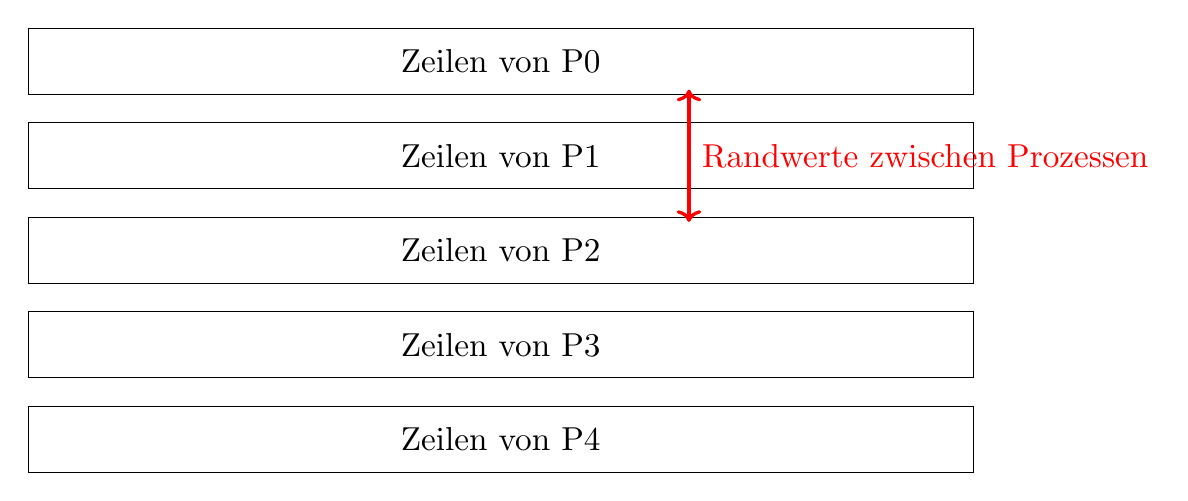
\begin{tikzpicture}[scale=1.2, every node/.style={scale=1.2}]
\foreach \i in {0,1,2,3,4} {
    \node[draw, minimum width=10cm, minimum height=0.7cm, anchor=west] (P\i) at (0, -\i) {Zeilen von P\i};
}
\draw[red, very thick, <->] (7, -0.3) -- (7, -1.7) node[midway, right, text=red] {Randwerte zwischen Prozessen};
\end{tikzpicture}
\end{center}

Das Diagramm zeigt die Kommunikation zwischen den Prozessen. Es werden blockierende und nicht-blockierende Kommunikation verwendet.

\begin{center}
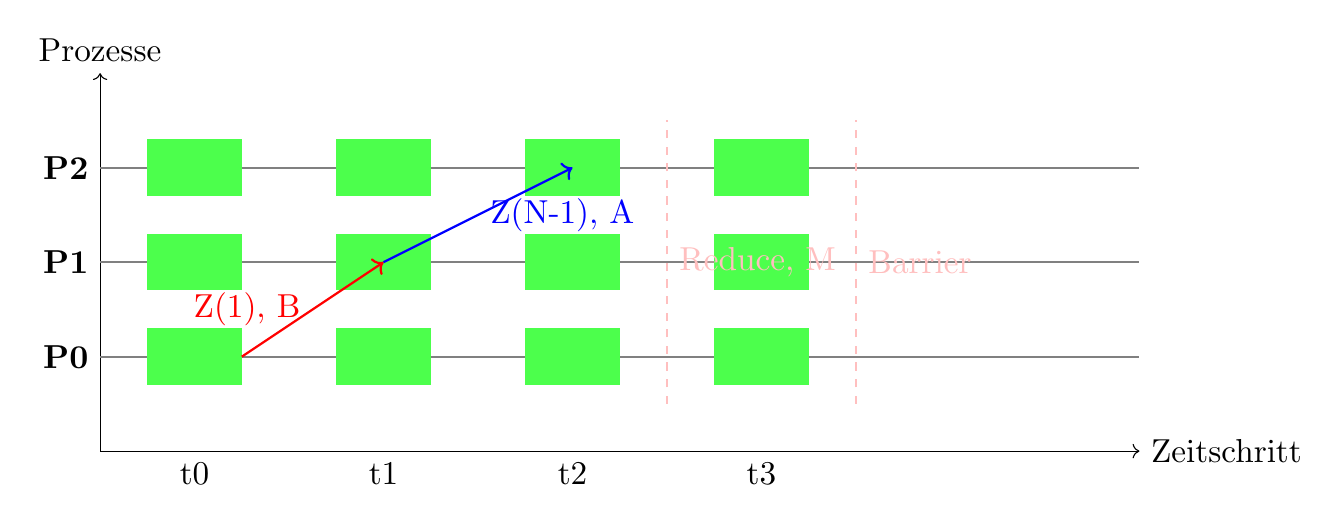
\begin{tikzpicture}[scale=1.2, every node/.style={scale=1.2}]
\draw[->] (0, 0) -- (11, 0) node[right] {Zeitschritt};
\draw[->] (0, 0) -- (0, 4) node[above] {Prozesse};
\foreach \y/\name in {1/P0, 2/P1, 3/P2} {
    \draw[thick, gray] (0, \y) -- (11, \y);
    \node[left] at (0, \y) {\textbf{\name}};
}
\foreach \x/\t in {1/t0, 3/t1, 5/t2, 7/t3} {
    \node[below] at (\x, 0) {\t};
}
\foreach \x/\y/\text in {0.5/1/t0, 2.5/1/t1, 4.5/1/t2, 6.5/1/t3, 0.5/2/t0, 2.5/2/t1, 4.5/2/t2, 6.5/2/t3, 0.5/3/t0, 2.5/3/t1, 4.5/3/t2, 6.5/3/t3} {
    \fill[green!70] (\x, \y-0.3) rectangle (\x+1, \y+0.3) node[midway] {\text};
}
\draw[red, thick, ->] (1.5, 1) .. controls (2.25, 1.5) .. (3, 2) node[midway, left] {Z(1), B};
\draw[blue, thick, ->] (3, 2) .. controls (4, 2.5) .. (5, 3) node[midway, right] {Z(N-1), A};
\draw[dashed, thick, pink] (6, 0.5) -- (6, 3.5) node[midway, right] {Reduce, M};
\draw[dashed, thick, pink] (8, 0.5) -- (8, 3.5) node[midway, right] {Barrier};
\end{tikzpicture}
\end{center}

Herausforderungen bei der Parallelisierung:

\begin{itemize}
    \item Lastenverteilung: Ungleichmäßige Verteilung bei nicht teilbarer Matrixgröße.
    \item Kommunikationsaufwand: Häufige Randwertaktualisierungen erfordern effiziente Methoden.
    \item Synchronisation: Barrieren und Reduktionen sind nötig, um konsistente Daten zu gewährleisten.
    \item Speicherzugriffe: Effizienter Umgang mit geteiltem und lokalem Speicher.
\end{itemize}

Optimierungsmöglichkeiten:

\begin{itemize}
    \item Block-Decomposition: Matrix in Blöcke aufteilen zur Reduzierung des Kommunikationsaufwands.
    \item Nicht-blockierende Kommunikation: Minimierung des Warteaufwands durch gleichzeitige Berechnungen und Kommunikation.
    \item Reduzierung von Barrieren: Weniger Synchronisation steigert die Leistung.
    \item Asynchrone Reduktionen: Maximierung des Parallelismus.
\end{itemize}

\end{document}
